\section{必修一知识点回顾【注意应用的数学思想:分类讨论、数形结合、变量替换】}
\startexercise
\chapter{例子}
\begin{exercise}
\item (17-18福州八中高一期中4)函数$f(x)=a^{-x^2+3x+2}(0<a<1)$的单调递增区间是\xz
        \xx{$(-\infty,\frac32)$}
        {$(\frac32,+\infty)$}
        {$(-\infty,-\frac32)$}
        {$(\frac32,+\infty)$}
\begin{answer}
不行吗。
\end{answer}
\item  (17-18福州八中高一期中5) 下列四组函数中,表示同一函数的是\xz
        \xx{$f(x)=\lg{x^4},g(x)=4\lg x$}
        {$f(x)=\sqrt{x+1}\cdot\sqrt{x-1},g(x)=\sqrt{x^2-1}$}
        {$f(x)=\frac{x^2-1}{x-1},g(x)=x+1$}
        {$f(x)=\begin{cases}x,x\geq0\\-x,x<0\end{cases},g(x)=\sqrt{x^2}$}
\begin{answer}
D
\end{answer}
\end{exercise}


\begin{enumerate} 
        \item[一、] 选择题请把......
        \item (17-18福州八中高一期中4)函数$f(x)=a^{-x^2+3x+2}(0<a<1)$的单调递增区间是\xz
        \xx{$(-\infty,\frac32)$}
        {$(\frac32,+\infty)$}
        {$(-\infty,-\frac32)$}
        {$(\frac32,+\infty)$}
        \begin{answer}
            D
        \end{answer}

        
        \item 等下写选择题小题内容 
        \item 等下写选择题小题内容 
        \item 等下写选择题小题内容 
        \item 等下写选择题小题内容 
        \item 等下写选择题小题内容 
        \item 等下写选择题小题内容 

        \item[二、] 填空题  ......
        \item (17-18八中高一期中11)若幂函数$f(x)$的图象过点$(2,\frac{\sqrt2}2)$ ,则$f(\frac14 )= $ \tk.
        \item 等下写填空题小题内容 
        \item 等下写填空题小题内容 
        \item 等下写填空题小题内容 
        \item 等下写填空题小题内容 

        \item[三、] 解答题  ......
        \item (福建省师大附中 2015-2016 高一上学期期中考试22)已知函数$f(x)=-1+\log_a{x+2}$($a>0$,且 $a \neq1$),$g(x)=(\frac12)^{x-1}$.\\
(1)函数$ y= f (x )$ 的图象恒过定点 $A$,求 $A$ 点坐标;\\
(2)若函数 $F ( x )= f ( x )- g ( x )$ 的图像过点$(2,\frac12)$, 证明:方程 $F ( x )= 0$ 在 $x\in(1,2)$上有唯一解. 


        \item 等下写解答题小题内容 
        \item 等下写解答题小题内容 
        \item 等下写解答题小题内容 
        \item 等下写解答题小题内容 
        \item 等下写解答题小题内容 
\end{enumerate} 

\item
(17-18八中高一期中19)已知$f(x)$是奇函数并且是$\mathbb{R}$上的单调函数,若函数$y=f(2x^2+1)+f(\lambda-x) $只有一个零点,则实数$\lambda $的值是\xz
\xx{$\frac14 $}{$\frac18 $}{$-\frac78 $}{$-\frac38 $}
\begin{answers}
C
\end{answers}

\item
(17-18三中高一上期中考12)已知$f(x)=\begin{cases}
 |\log_3x|,0<x\leq3\\13-4x,x>3   
\end{cases} $ ,若正数$a$ ,$b$ , $c$互不相等,且$f(a)=f(b)=f(c)$ ,则$abc$ 的取值范围是\xz
\xx{$(3,13)$}{$(\frac14,13) $}{$(1,\frac{13}{4}) $}{$(3,\frac{13}{4})$}
\begin{answers}
D
\end{answers}

\item
(17-18三中高一上期中考10)已知函数$f(x)$ 为$\mathbb{R}$ 上的奇函数,$f(x)$ 在$(0,+\infty)$ 内单调递减,且存在$x_0<0$ 使得 $f(x)=0$,则函数$f(x)$ 的零点个数为\xz\\
\xx{1个}{2个}{3个}{4个}
\begin{answers}
C
\end{answers}
\item
(17-18八中高一期中20)若函数$f(x)=|2^x-1|-b $有两个零点,则实数$b$的取值范围是\tk.\\


%福州重点中学期中考真题分类汇编 2函数的相关性质.pdf P5.7
\item(福建师大附中 16-17 高一期中考,7)已知定义在 $\mathbb{R}$上的函数$f(x)$在 $(-\infty,2)$内为减函数,且$f(x+2) $为偶函数,则$f(-1)$,$f(4)$,$f(\frac{11}2 )$的大小为\xz \\
\xx{$f(4)<f(-1)<f(\frac{11}2 )$}
	   {$f(-1)<f(4)<f(\frac{11}2 )$}
       {$f(\frac{11}2 )<f(4)<f(-1)$}
       {$f(-1)<f(\frac{11}2 )<f(4)$}
\begin{answer}A\end{answer}\\
     
\item
%福州重点中学期中考真题分类汇编 2函数的相关性质.pdf P6.9\\
(福州高级中学 16-17 高一期中考,13)已知函数$f(x)=\sqrt{x^2+ax+a} $ 在区间$[1,+\infty] $上单调递增,则实数$a$的取值范围是\xz\\
\xx{$[-2,-\frac12]$}
		{$[-\frac12,+\infty] $}
        {$[-\frac12,2] $}
        {$[-2,+\infty] $}
\begin{answer}B\end{answer}

\item
(17-18三中高一上期中考16)已知函数$f(x)=(\log_427)^2+2a\log_2x+1 $ 有大于 1的零点,则实数$a$ 的取值范围是\tk.
\begin{answers}
$(-\infty,-1]$
\end{answers}


\item
%福州重点中学期中考真题分类汇编 2函数的相关性质.pdf P8.9\\
(福建师大附中 16-17 高一期中考,16)函数$f(x)$ 是$(0,+\infty)$ 上的单调增函数,当 $n\in \mathbb{N}^*$ 时,$f(n)\in\mathbb{N}^*$ ,且 $f[f(n) ] =3n$,则$f(1)$ 的值为\tk.\\
\begin{answers}2\end{answers}


\item
%福州重点中学期中考真题分类汇编 2函数的相关性质.pdf P6.13\\
(福州格致中学 16-17 高一期中考,10)若$f(x)=-x^2+2ax $
 与$g(x)=\frac a{x+1} $在区间$[1,2] $上都是减函数,则实数$a $ 的取值范围\xz\\
 \xx{$(-1,0)\cup (0,1) $ }
 		{$(-1,0)\cup (0,1]$}
        {$(0,1) $}
        {(0,1]}
 \begin{answer}      D\end{answer}

\item
%福州重点中学期中考真题分类汇编 2函数的相关性质.pdf P7.7\\
(福建师大附中 16-17 高一期中考,14)已知函数 $f(x)$ 的反函数是 $y=\frac{1}{3^x}$,则函数 $f(2x-x^2) $的减区间为\tk

\item
%福州重点中学期中考真题分类汇编 2函数的相关性质.pdf P8.12\\
(福州格致中学 16-17 高一期中考,15)若函数$f(x)=\begin{cases}(a-2)x,x\leq2\\(\frac{1}{2})^x-1,x<2\end{cases}$是$\mathbb{R}$上的单调递减函数,则实数$a$的取值范围是\tk.
\begin{answers}
$a\leq\frac{13}{8}$
\end{answers}

%福州三中高一上数学七中卷(2017-2018).doc
\item
(17-18三中高一上期中考19)(本小题满分 分)\\
已知函数$f(x)=\sqrt{ax+4}$ $(a\in\mathbb{R},a\neq0)$  .\\
(I)若$a=-1$ ,求函数$f(x)$ 的定义域和值域;\\  
(II)若$f(x)$ 在区间$[-1,2] $ 上为单调函数,求实数$a$ 的最大值和最小值.\\
\begin{answers}
(I)定义域$(-\infty,4]$,值域$[0,+\infty)$;
(II)$a_{\min}=-2,a_{\max=4} $.
\end{answers}





\item
(17-18八中高一期中22)(本小题共12分)
已知函数$f(x)=x^2+4ax+2a+6 $.\\
(I)若函数$y=\log_2f(x)$的最小值为2,求$a$的值;\\
(II)若对任意$x\in\mathbb{R}$,都有$f(x)\geq0$成立,求函数$g(a)=2-a|a+3| $的值域.\\

\item
%福州重点中学期中考真题分类汇编 4函数方程及函数模型的应用.pdf P6
(16-17 附中21) 为了研究某种药物,用小白鼠进行试验,发现药物在血液内的浓度与时间的关系因使用方式的不同而不同。若使用注射方式给药,则在注射后的 3 小时内,药物在白鼠血液内的浓度$y_1$与时间$t$ 满足关系式:$y_1 =4-at$ ($0<a<\frac{4}{3})$,$a$为常数),若使用口服方式给药,则药物在白鼠血液内的浓度 $y_2$与时间 $t$满足关系 式:$y_2=\begin{cases}\sqrt{t},0<t<1,\\3-\frac{2}{t},1\leq t\leq3.\end{cases}$现对小白鼠同时进行注射和口服该种药物,且注射药物和口服药物的吸收与代谢互不干扰.\\
(Ⅰ)若$a=1$,求 3 小时内,该小白鼠何时血液中药物的浓度最高,并求出最大值;\\
(Ⅱ)若使小白鼠在用药后 3 小时内血液中的药物浓度不低于 4,求正数 $a$ 的取值范围.\\
\begin{answers}
(1)当$t=\frac12$时,$y_{\max}=\frac{17}{4}$;\\
(2)$0<a\leq\frac{7}{9}$
\end{answers}


\item
(17-18八中高一期中23)(本小题共15分)
已知二次函数$f(x)$满足$f(x+1)-f(x)=2x $ $(x\in\mathbb{R})$,且$f(0)=1$.\\
(I)求$f(x)$的解析式;\\
(II)若函数$g(x)=f(x)-2tx$在区间$[-1,5]$上是单调函数,求实数$t$的取值范围;\\
(III)若关$x$的方程$f(x)=x+m $在区间$(-1,2)$上有唯一实数根,求实数$m$的取值范围.(注:相等的实数根算一个).\\

%福州重点中学期中考真题分类汇编 2函数的相关性质.pdf P9
\item (福建省师大附中 2015-2016 高一上学期期中考试22)已知函数$f(x)=-1+\log_a{x+2}$($a>0$,且 $a \neq1$),$g(x)=(\frac12)^{x-1}$.\\
(1)函数$ y= f (x )$ 的图象恒过定点 $A$,求 $A$ 点坐标;\\
(2)若函数 $F ( x )= f ( x )- g ( x )$ 的图像过点$(2,\frac12)$, 证明:方程 $F ( x )= 0$ 在 $x\in(1,2)$上有唯一解.
\begin{answer}
(1)$(-1,-1)$;\\
\end{answer}

%福州重点中学期中考真题分类汇编 2函数的相关性质.pdf P10
\item (福建省师大附中 2015-2016 高一上学期期中考试23) 已知函数 $f ( x ) =\log_a ( x+ 1), g ( x )= 2 \log_a ( 2 x+ t )(t\in \mathbb{R})$, $a> 0$, 且$a\neq 1$.\\
(\Rmnum{1})若 1 是关于 $x$ 的方程 $f ( x) -g ( x) =0$ 的一个解,求 $t$ 的值;\\
(\Rmnum{2})当 $0< a< 1$且$t=-1$ 时,解不等式 $f ( x)\leq g ( x) $;\\
(\Rmnum{3})若函数 $F ( x)= a^{f ( x ) }+ tx^2- 2t+ 1 $在区间 $(-1,2]$上有零点,求 $t$ 的取值范围.
\begin{answer}
(\Rmnum{1})$t=\sqrt{2}-2$;
(\Rmnum{2})$x\in(\frac12,\frac54]$;
(\Rmnum{3})$t\in(-\infty,2]\cup [\frac{2+\sqrt{2}}{4},+\infty)$.
\end{answer}

\item
%福州重点中学期中考真题分类汇编 2函数的相关性质.pdf P11
(福州八中 2015—2016 高一上学期期中考试23)设 $f (x )$ 是定义在 $\mathbb{R}$ 上的奇函数,且对任意 $a,b\in \mathbb{R}$ ,当$a+b\neq0$时,都有 $\frac{f(a)+f(b)}{a+b}>0$\\
(1)若 $a> b$ ,试比较 $f (a ) $与 $f (b)$ 的大小关系;\\
(2)若 $f (9^x- 2\cdot 3^x )+ f ( 2\cdot 9^x-k )> 0 $对任意 $x\in[0,\infty )$ 恒成立,求实数 $k$ 的取值范围.
\begin{answer}
(1)$f(a)>f(b)$;\\
(2)$k<1$.\\
\end{answer}

%福州重点中学期中考真题分类汇编 2函数的相关性质.pdf P12
(福州八中 2015—2016 高一上学期期中考试24)已知函数 $y=x+\frac tx$ 有如下性质:如果常数 $t>0$,那么该函数在$(0,\sqrt t]$上是减函数, 在$[\sqrt t, +\infty)$上是增函数.\\
(1)已知 $f(x)=\frac{4x^2-12x-3}{2x+1} $,$x\in[0,1]$,利用上述性质,求函数 $f(x)$的单调区间和值域;\\
(2)对于(1)中的函数 $f(x)$和函数$g(x)=-x-2a$,若对任意 $x_1 \in[0,1]$,总存在 $x_2\in[0,1]$,使得 $g(x_2 )=f(x_1 ) $成立,求实数 $a$ 的值.


%福州重点中学期中考真题分类汇编 2函数的相关性质.pdf P14
(福州市第三中学 2016-2017 高一上期中考试23)设函数 $f (x)=a^x+ bx +c$ ( $a> 0$ , $b, c\in \mathbb{R})$ . \\
⑴若 $f (1)= c$ , $f (x)$在$( k,+\infty)$单调递增,求实数 $k$ 的取值范围;\\
 ⑵若 $f( 1)=-\frac a2$,求证:函数 $f (x) $在$( 0,2) $内至少有一个零点.


%福州重点中学期中考真题分类汇编 2函数的相关性质.pdf P16
(福建师大附属中学 2016-2017 高一年级期中考试22)已知二次函数 $f ( x )= ax^2+ bx+ c$ 的图像过点 $(-2,0)$ ,且不等式 $2 x\leq f ( x )\leq \frac12x^2+ 2$ 对一切实数 $x$ 都成立.\\
(\Rmnum{1})求函数 $f ( x ) $的解析式. \\
(\Rmnum{2}成立,求实数 $t$ 的取值范围.


%福州重点中学期中考真题分类汇编 2函数的相关性质.pdf P16
(福州市高级中学 2016-2017 高一上期中19)已知 $f(x)$是定义在$\mathbb{R}$上的奇函数,当$x\geq0$时,$f(x)=a^x-2$,其中 $a> 0$ 且 $a\neq 1$\\
(I)求 $f (x )$ 的解析式;\\
(II)解关于$x$ 的不等式 $-1< f(x)<4$ ,结果用集合或区间表示.


%福州重点中学期中考真题分类汇编 2函数的相关性质.pdf P17
(福州市高级中学 2016-2017 高一上期中21)记函数 $f (x )=a-\log_2{x}(1\leq x\leq 4)$,函数$y=[f(x)]^2-f(\frac x2)$,记函数$f(x)$ 的最小值为 $g( a)$.\\
(I)求 $g( a) $的表达式;\\
(II)作出函数$y=|g(a)|$的图像,并根据图像回答:当 $k$ 为何实数时,方程$|g( a)|-k=0$ 有两个解、有四个解、有无穷多个解?

%福州重点中学期中考真题分类汇编 2函数的相关性质.pdf P19
(福州市高级中学 2016-2017 高一上期中22)已知函数$f(x)=x^2-2ax+5(a>1)$\\
(I)若 $f (x )$ 的定义域和值域均是 $[1, a]$ ,求实数 $a$ 的值; \\
(II)若 $f (x ) $在区间 $[4,+\infty)$上是增函数,且对任意的$ x \in[1, a+ 2]$,都有 $f( x )\leq 0$ ,求实数$a$的取值范围;\\
(III)若 $g( x )=2^x+\log_2{x+ 1 }$ ,且对任意的 $x \in[0,1]$ ,都存在$f(x_0)=g(x)$ 成立,求实数$a$的取值范围.


%福州重点中学期中考真题分类汇编 2函数的相关性质.pdf P21
(福州市格致中学 2016-2017 高一上期中考试数学学科试卷22)已知二次函数 $f ( x )= ax^2+ bx+3$ 是偶函数,且 过点$(-1,4)$,$ g ( x )= x + 4$ .\\
(Ⅰ)求 $f (x) $的解析式;\\
()求函数 $F ( x )= f (2^x )+ g (2^{x+1} )$ 的值域; \\
(Ⅲ)若 $f ( x ) \geq g ( mx +m )$ 对 $x\in [2, 6] $恒成立,求实数 $m$ 的取值范围.

\subsection{集合是什么?怎么表示?有什么性质?记住一些特殊的集合及其表示方法、性质。}
    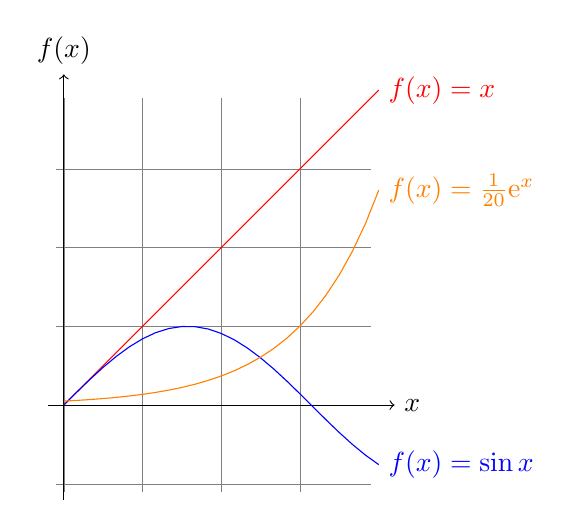
\begin{tikzpicture}[domain=0:4]
  \draw[very thin,color=gray] (-0.1,-1.1) grid (3.9,3.9);
  \draw[->] (-0.2,0) -- (4.2,0) node[right] {$x$};
  \draw[->] (0,-1.2) -- (0,4.2) node[above] {$f(x)$};
  \draw[color=red]    plot (\x,\x)             node[right] {$f(x) =x$};
  % \x r 表示弧度
  \draw[color=blue]   plot (\x,{sin(\x r)})    node[right] {$f(x) = \sin x$};
  \draw[color=orange] plot (\x,{0.05*exp(\x)}) node[right] {$f(x) = \frac{1}{20} \mathrm e^x$};
\end{tikzpicture}
\subsection{集合间有什么关系?注意与一些特殊集合间的关系。}

\begin{enumerate}
\item 集合间的运算: 交集、并集、补集的含义与表示。运算结果有何特殊性质? 
\end{enumerate}

\begin{enumerate}
\item  计算二重积分~$\ds{\iint\limits_{D}\me^{x^2+y^2}\dif \sigma}$, 其中~$D=\{(x,y)\Big| x^2+ y^2 \leqslant 25\}$.\\
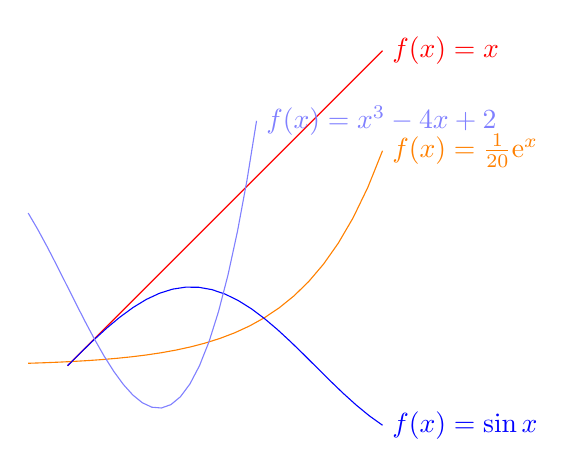
\begin{tikzpicture}[domain=0:4]
\tkzInit[xmax=4.2,ymax=3.2,xmin=-1.2,ymin=-1.2,xstep=1]
%\tkzGrid
\tkzAxeXY
\draw[color=red] plot (\x,\x) node[right] {$f(x)=x$};
\draw[color=orange,domain=-0.5:4] plot (\x,{0.05*exp(\x)}) node[right] {$f(x)=\frac{1}{20}\mathrm e^x$};
\draw[color=blue,domain=0:4] plot (\x,{sin(\x r)}) node[right] {$f(x)=\sin x$};
\draw[color=blue!50,x=1cm,y=0.5cm,domain=-0.5:2.4] plot (\x, {(\x)^3-4*(\x)+2}) node[right] {$f(x)=x^3-4x+2$};
\end{tikzpicture}
\end{enumerate}


集合的应用。集合与其他数学概念的联系。

函数是什么?怎么表示?有什么性质?记住一些特殊的函数及其表示方法、性质。\\
指数幂如何表示与计算?运算规则如何?与已学过运算间的联系?\\
对数如何表示与计算?运算规则如何?与已学过运算间的联系?

函数间有什么关系?

函数间的运算:加减乘除、复合的含义与表示。运算结果有何特殊性质?

函数的应用。函数与其他数学概念的联系。

二、运算与技巧
几种常用的表达式化简与处理办法\\
函数是什么?怎么表示?有什么性质?记住一些特殊的函数及其表示方法、性质。\\
指数幂如何表示与计算?运算规则如何?与已学过运算间的联系?\\
对数如何表示与计算?运算规则如何?与已学过运算间的联系?
几种方程与不等式的求解办法

几种常见问题含义

\chapter{例子}
\begin{exercise}
\item 题目
\begin{answer}
这有答案。
\end{answer}
\item 又一道
\begin{answer}
这还有答案。
\end{answer}
\end{exercise}
%\stopexercise
%\startexercise
\begin{exercise}
  \item 是的
  \item 哦也
  \begin{answer}

\end{answer}
\end{exercise}
\stopexercise

\chapter{答案}
\printanswer









